\documentclass[../main.tex]{subfiles}
\begin{document}
\chapter{Boolesche Funktionen}\label{chp:surreal}
\section{Zahlendarstellung}
  \begin{itemize}
    \item $\sum$: ein fest gewähltes Input Alphabet
    \item $\sum^n$: ein Wort der Länge $n$ über $\sum$
    \item $\sum_b := \{0,\ldots,b-1\}$: Alphabet des b-adischen Zahlensystems ($b<1$)\newline
    \begin{examples}
        \begin{itemize}
            \item[-] $\sum_2=\{0,1\}$: Dual oder Binäralphabet
            \item[-] $\sum_8 = \{0,1,2,3,4,5,6,7\}$: Oktalalphabet
            \item[-] $\sum_10 = \{0,1,2,3,4,5,6,7,8,9\}$: Dezimalalphabet
        \end{itemize}
    \end{examples}
\end{itemize}
  \subsection{b-adische Darstellung natürlicher Zahlen}
  \begin{definition}
    Sei $b \in \mathbb{N}$ mit $b > 1$. Dann ist jede natürliche Zahl $z$ mit 
    $0\leq z \geq b^n-1$ (und $n \in \mathbb{N}$) eindeutig als Wort der Länge $n$ über $\sum_b$ darstellbar durch:
    \[ z =\sum_{i=0}^{n-1} z_ib^i = z_0b^0+z_1b^1 + \ldots + z_{n-1}b^{n-1} \]
    mit $z_i \in \sum_b = \{0,\ldots,b-1\}$ für $i = 0,\ldots,n-1$\dots
  \end{definition}
  Als vereinfachende Schreibweise ist dabei folgende $Ziffernschreibweise$ üblich;
  \[z = \(z_{n-1}z{n-2}\ldots z_1z_0\)_b\]
  Wichtiger Spezialfall: $b = 2$ ("Dualdarstellung" natürlicher Zahlen)
  \begin{examples}
    \[\(26\)_10 = 2*10^1+6*10^0=2*10+6*1 = 20+6\]
    \[\(11010\)_2=1*2^4+1*2^3+0*2^2+1*2^1+0*2^2 = 1*16+1*8+0*4+1*2=16+8+2\]
    \[\(1A\)_16= 1*16^1+10*16^0 = 1*16+10*1 = 16+10\]

  \end{examples}
\section{Addition}
-Dezimaladdition\ \ \ \ \ \ -Binäraddition\newline
\begin{verbatim}
   183               10110111
  +197              +11000101
   11               1    111
   ---              ---------
   380              101111100
\end{verbatim}
\section{Schaltfunktion}
\begin{definition}
    Seien $n,m \in \mathbb{N}, n,m \leq 1$. Dann heisst eine Funktion $F: B^n \rightarrow B^m$ Schaltfunktion.
\end{definition}
\begin{examples}\newline
    \begin{itemize}
        \item Addition von zwei 16-stelligen Dualzahlen
        \[A: B^{32} \rightarrow B^{17}\]
        \item Multiplikation von zwei 16-stelligen Dualzahlen
        \[M: B^{32} \rightarrow B^{32}\]
        \item Sortieren von 30 16-stelligen Dualzahlen
        \[S: B^{480} \rightarrow B^{480}\]
        \item Primzahltest
        \[P: B^{32} \rightarrow B,\ mit\ P(x)=1,\ falls\ x\ Primzahl\ ist,\ 0\ sonnst.\]
    \end{itemize}
\end{examples}
\section{Boolesche Funktionen}
\begin{definition}
    Eine Schaltfunktion $f : B^n \rightarrow B$ heisst ($n$-stellige) Boolesche Funktion.
    $Zusammenhang\ zu\ Schaltfunktionen:$ \newline
    Sei $F:B^n\rightarrow B^m$ mit $F(x_1,\ldots,x_n) = (y_1,\ldots,y_n)$. Setzt man für jedes $i \in \{1,\ldots,m\}$
    \[f_i : B^n \rightarrow B,\]
    def. durch
    \[ f_i(x_1,\ldots,x_n) = y_i,\]
    so ist $F$ wie folgt darstellbar:
    \[F(x_1,\ldots,x_n)=(f_1(x_1\ldots x_n),f_2(x_1 \ldots x_n),\ldots,f_m(x_1,\ldots,x_n))\]
    für alle $x_1,\ldots,x_n \in B$.
\end{definition}
\subsection{1-stellige Boolesche Funktionen}
\begin{tabular}[h]{l|c|r|t|z}
    $x$ & $f_0(x)$ & $f_1(x)$ & $f_2(x)$ & $f_3(x)$ \\
    \hline
    0 & 0 & 0 & 1 & 1\\
    \hline
    1 & 0 & 1 & 0 & 1 \\
\end{tabular}
\newline    
Es gilt: $f_0(x)=0, f_1(x) = x, f_2(x) =\bar{x}, f_3(x)=1$ \newline
Die Funktion $f_2(x)$ wird auch als NOT(x) und ¬x bezeichnet.
\subsection{2-stellige Boolesche Funktionen}
%\begin{tabular}[h]{c|c|c|c|c|c|c}
 %   x & y & AND & OR & XOR & NAND & NOR\\
 %     &   & Konjunction & Disjunktion & Exclusive OR & Not And & Not Or \\
 %     &   & \land & \lor & \nleftrightarrow & ¬AND & ¬OR\\
 %     &   & $f_1$ & $f_7$ & $f_6$ & $f_{14}$ & $f_8$\\\hline
 %   0 & 0 & 0 & 0 & 0  & 1 & 1\\\hline
 %   0 & 1 & 0 & 1 & 1  & 1 & 0\\\hline
 %   1 & 0 & 0 & 1 & 1  & 1 & 0\\\hline
 %   1 & 1 & 1 & 1 & 0  & 0 & 0\\
%\end{tabular}
%\newline
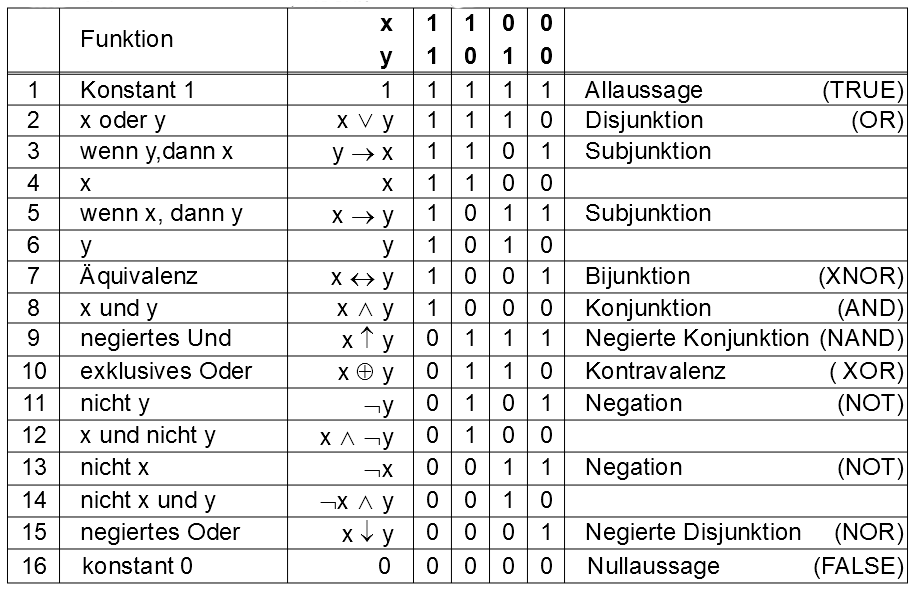
\includegraphics[width=\textwidth]{02-2boolesche}
\subsection{Gesetze einer Booleschen Algebra}
\begin{itemize}
\item Kommuntativgesetze: $x \lor y = y \lor x, x \land y = y \land x$
\item Assoziativgesetze: $(x \lor y) \lor z = x \lor (y \lor z),
(x \land y) \land z = x \land (y \land z)$
\item Verschmelzungsgesetze: $(x \lor y) \land x = x,(x \land y) \lor x = x$
\item Distributivgesetze: $x \land (y \lor z)=(x \land y) \lor (x \land z),
x \lor (y \land z)=(x \lor y) \land (x \lor z)$
\item Komplementgesetze: $x \lor (y \land y) = x, x \land (y \lor y) = x$
\item Neutrale Elemente 0, 1: $x \lor 0 = x, x \land 0=0, x \land 1 = x, x \lor 1=1$
\item de Morgansche Regeln: $\overline{x \lor y} = \bar{x} \land \bar{y}, \overline{x \land y} = \bar{x} \lor \bar{y}$
\item Idempotenz: $x = x \lor x = x \land x = \bar{\bar{x}}$
\end{itemize}
\begin{example}
\[¬((¬a*c)+(¬a*d)) ¬a\ ausklammern\ (Distributivgesetz)\]
\[=¬(¬a*(C+d))\ de\ Morgan \]
\[=¬¬a * ¬(c+d)\ Idempotenz \]
\[=a + ¬(C+d)\ de\ Morgan \]
\[=a+(¬c*¬d) \]
\end{example}
\subsection{Bedeutung von Booleschen Algebren}
Boolesche Algebren kommen in verschiedenen mathematischen
Teilgebieten vor. Ihre Bedeutung ist nicht nur auf die technische
Informatik beschränkt.
\begin{examples}
\begin{itemize}
    \item Boolesche Ringe (Algebra)
    \item Verbände (Ordnungstheorie)
    \item Kompakte, total unzusammenhängende Hausdorfräume (Topologie)
    \item Semantik für Logiken
    \item Boolean-valued models (Modelltheorie, gängiges Mittel um die Unabhängigkeit der Kontinuumshypothese von ZFC zu zeigen)
\end{itemize}
\end{examples}
\subsection{Boolesche Körper}
Die Menge B = \{0,1\} mit den Operationen XOR und AND bildet
einen Körper mit dem Nullelement 0 und dem Einselement 1.
In dem Zusammenhang wird XOR als Addition (+) und AND als
Multiplikation (*) betrachtet.
\newline
\begin{goals}
\begin{enumerate}
    \item Sie können Zahlen zwischen verschiedenen Zahldarstellungen umrechnen
    \item Sie kennen die Begriffe Schaltfunktion und Boolesche Funktion
    \item Sie kennen alle ein- und zweistellige Boolesche Funktionen
    \item Sie können für eine zusammengesetzte Boolesche Funktion die
    Wahrheitstabelle berechnen
    \item Sie kennen die Gesetze der Boolesche Algebra und können diese
    verwenden, um Boolesche Ausdrücke umzuformen
    \item Sie können überprüfen, ob zwei Boolesche Ausdrücke dieselbe Funktion
    beschreiben (sowohl durch Ausrechnen als auch durch Umformen).
    
\end{enumerate}
\end{goals}
\end{document}